%Input preamble
\documentclass[11pt]{article}

% colors
\usepackage[table]{xcolor}
\definecolor{maroon}{RGB}{153,0,18}
\definecolor{lime}{RGB}{190,213,88}
\definecolor{sand}{RGB}{217,202,179}
\definecolor{fire}{RGB}{144,50,61}
\definecolor{brick}{RGB}{94,11,21}
\definecolor{olive}{RGB}{117,109,84}
\definecolor{lavpink}{RGB}{172,123,132}
\definecolor{darkpurp}{RGB}{49,10,49}
\definecolor{salmon}{RGB}{204,90,113}
\definecolor{mauve}{RGB}{94,73,85}
\definecolor{greyblue}{RGB}{125,132,145}
\definecolor{greypurp}{RGB}{68,56,80}
\definecolor{brightpurp}{RGB}{96,20,255}

% packages (please add in alphabetical order)
\usepackage{adjustbox}
\usepackage{amsfonts}
\usepackage{amsmath}
\usepackage{amssymb}
\usepackage{array}
\usepackage{bm}
\usepackage{booktabs}
\usepackage{caption}
\usepackage{epstopdf}
\usepackage{float}
\usepackage[margin=1in]{geometry}
\usepackage{graphicx}
\usepackage[colorlinks=true, linkcolor=brightpurp, citecolor=brightpurp, urlcolor=salmon]{hyperref}
\usepackage{lipsum}
\usepackage{longtable}
\usepackage{mathtools}
\usepackage{multirow}
\usepackage{natbib}
\usepackage{rotating}
\usepackage{setspace}
\usepackage{subcaption}
%\usepackage{threeparttable}
\usepackage{threeparttablex}
\usepackage{xr}
\usepackage[printwatermark]{xwatermark}


\newcolumntype{L}[1]{>{\raggedright\let\newline\\\arraybackslash\hspace{0pt}}m{#1}}
\newcolumntype{C}[1]{>{\centering\let\newline\\\arraybackslash\hspace{0pt}}m{#1}}
\newcolumntype{R}[1]{>{\raggedleft\let\newline\\\arraybackslash\hspace{0pt}}m{#1}}

% commands
\newcommand{\mr}{\multirow}
\newcommand{\mc}{\multicolumn}


\begin{document}

\noindent This section of the appendix assess some of the critiques to ABC, which could apply to CARE as well. This focus on the first phase of the program, to which we refer simply as ABC in this section of the appendix.\\

\noindent \citet{} asks if ABC prevented socio-cultural mental retardation. He focuses on different measures of cognition, and generically calls them IQ. His main focus is on the difference raw mean difference in the Bayley Mental Development Index (MDI) at age 1.\footnote{The Bayley Mental Development Index is a standard measure of cognition at taken between ages 0 and 2 \citep{•}.} He finds a noticeable difference in the mean difference between cohorts 1 and 2 and cohorts 2 and 4, as early as six months after the treatment began. As \citet{} argues, this difference is conspicuous and we display it in Table~\ref{tab:}.\\

\noindent \citet{} suggests some possibilities: ``an essential question is whether the differences at 6 months of age were due to the intervention or where preexisting (p. 230)''. \citet{} proceeds with speculative exercises that lead him to conclude that it is questionable to conclude that the mean difference between the treatment and control groups as early as age six months is a consequence of the treatment.\footnote{The exact quote is: ``Even if the differences between experimental and control groups at 6 months of age were a consequence of the first few months of intervention, which is questionable, the negligible additional effects after age 4.5 more years in the program should at least make one cautious about this kind of intervention's potential [\ldots] We asses the former point before getting to the latter.''}\\

\noindent His argument oscillates from not receiving not receiving information on the maternal characteristics which he considers fundamental for his analysis to comparing test scores over the year, and tests scores \textit{do not have a well-defined scale}.\\ 

\noindent We make three annotations with respect to the comments in \citet{}.\\ 

\noindent First, when jointly testing the hypothesis of differences in a battery of observed characteristics, we fail to reject any difference between the families of these children (see Table~\ref{tab:baseline_coh3} and Table~\ref{tab:baseline_coh4}). Even when the point estimates present some differences, they are minimal. For example, treatment-group mother differ, on average, by having one more point in the IQ score, which has a population standard deviation of 15. This makes it less likely that there were some intrinsic differences between the treatment and control groups before randomization.\\

\noindent A more recent program, the Infant Health and Development Program (IHDP), treated children from ages 0 to 3. \citet{Gross_Spiker_etal_1997_BOOKHelpinglowbirth} thoroughly describe this program. A lots of its elements were based on ABC and CARE. The program offered an average of eight hours a week of center-based childcare from ages 1 to 3, weekly home visits from ages 0 to 1, and bi-monthly home visits from ages 1 to 3. Measures on the Bayley MDI at 12 and 24 months are available. The most intensive part of the treatment, center-based childcare, began at age 12 months in IHDP while it began at birth 0 in ABC. As in ABC, after a few months of center-based childcare, the effects on cognition were substantial in IHDP. This makes more likely possibility of treatment effects on measures of cognition to appear very early in life, for programs similar to ABC.\\

\noindent Second, when partialing out in a linear regression the score in the Bayley MDI tests both at six and twelve months of age, the treatment effects on IQ, measures by the mean difference between the treatment and the control groups, are still significant and are sustained up to age 21 (see Figure~\ref{fig:treatiqsabc}).

\begin{figure}[H]
		\caption{Treatment Effects on IQ, ABC} \label{fig:treatiqsabc}
		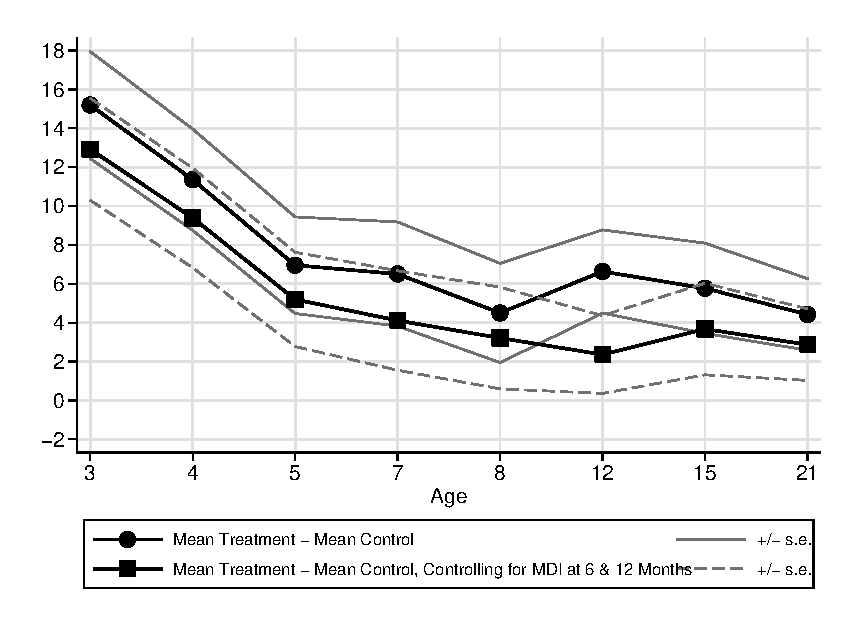
\includegraphics[width=.9\columnwidth]{output/abc_mdifixing_2.eps}
\floatfoot{
\footnotesize
\noindent Note: This figure displays the mean difference between the treatment and the control groups in IQ at different ages, pooling males ans females. The dotted line represents the raw difference. The squared line represents the difference when linearly controlling for the Bayley Mental Development Index at 6 and 12 months.}
\end{figure}

\end{document} 